\documentclass[11pt]{article}

\usepackage[left=2cm, right=2cm, top=2.5cm, bottom=2.5cm]{geometry}
\geometry{letterpaper}


\usepackage[x11names]{xcolor}
\usepackage{fancyhdr, amssymb, cancel, amsmath, graphicx, pgfplots, tikz}

\newcommand{\stylecolor}{black}

\usepackage[colorlinks=true, urlcolor=violet, linkcolor=blue, citecolor=red, hyperindex=true, linktocpage=true]{hyperref}




\usepackage[explicit]{titlesec}

\newcommand*\sectionlabel{}
\titleformat{\section}
  {\gdef\sectionlabel{}
   \Large\bfseries\scshape}
  {\gdef\sectionlabel{\thesection. }}{0pt}
  {\begin{tikzpicture}[remember picture,overlay]
	\draw (-0.2, 0) node[right] {\textsf{\sectionlabel#1}};
	\draw[thick] (0, -0.4) -- (\textwidth, -0.4);
       \end{tikzpicture}
  }
\titlespacing*{\section}{0pt}{15pt}{20pt}

\newcommand*\subsectionlabel{}
\titleformat{\subsection}
  {\gdef\subsectionlabel{}
   \large\bfseries\scshape}
  {\gdef\subsectionlabel{\thesubsection.\ \  }}{0pt}
  {\begin{tikzpicture}[remember picture,overlay]
    	\draw (-0.15, 0) node[right] {\textsf{\subsectionlabel#1}};
       \end{tikzpicture}
  }
\titlespacing*{\subsection}{0pt}{10pt}{10pt}

\pgfplotsset{every axis legend/.append style={at={(1.02,1)},anchor=north west}}

\newcommand{\titletext}{Parallel implementation of fast randomized algorithms for the decomposition of low rank matrices}

\renewcommand{\figurename}{\textsc{Figure}}
\renewcommand{\tablename}{\textsc{Table}}


\begin{document}

\pagestyle{fancy}
\renewcommand{\headrulewidth}{0pt}
\fancyhead{}

\fancyfoot{}
\fancyfoot[C] {\textsf{\textbf{\thepage}}}












\tableofcontents




\section{Introduction}
Computational mathematics and science increasingly involves calculations using very large matrices which may easily be hundreds of gigabytes in size.  Nonetheless, many fundamental matrix algorithms such as QR factorization are not only very slow, with flop complexities of  common, but also scale poorly on parallel machines due to frequent global communications.

A few years ago, it was proposed in a series of papers \cite{rokyale1, rokyale2, rokpnas} that a procedure, coined interpolative decomposition (ID), could decompose an  matrix, with approximate rank , into two much smaller matrices.  Furthermore, when using a probabilistic algorithm to perform the ID, one had quadratic scaling behavior and much of the algorithm could be naturally parallelized.   Performing an ID on a large low-rank matrix not only allows for it to be stored in a much smaller amount of memory, but it allows for many core operations (such as matrix multiplication) to run significantly faster.  Furthermore, the ID and similar randomized algorithms can serve as the basis for fast methods for the singular value decomposition (SVD) \cite{rokpnas} and principal component analysis \cite{rok1}, as well as tensor skeleton generalizations \cite{drineas} and least squares problems \cite{boutsidis, rok2, rudelson}; for a much more thorough list see \cite{martinsson}.

Although there is increasing interest in probabilistic algorithms, we are not aware of these algorithms having been tested on extremely large matrices where massive parallelization is essential.  In this paper, we present results obtained on a Cray XMT supercomputer by performing a randomized ID on matrices over 100 GB in size, which is two orders of magnitude larger than previous matrices studied (without making calls out of RAM).   In doing so, we confirm the conjecture that such algorithms can run efficiently in parallel, demonstrating that for many matrices, the algorithm's parallelism scales by at least two orders of magnitude.  We also confirm numerical results which suggested that the error bounds on the procedure grow slowly with matrix size, implying that these procedures are appropriate for high-precision computation on extremely large matrices.

\section{The Randomized Interpolative Decomposition Algorithm}
Let  be an  complex matrix with approximate rank , with .  By approximate rank, we mean that the  largest singular value, , is small. The goal of the randomized ID algorithm \cite{rokpnas} is to find an  matrix  and a  matrix  such that It is well-known from the Eckart-Young theorem \cite{eckart} that the best possible choices of  and  come from performing a spectral value decomposition (SVD)  replacing  with a truncated diagonal matrix  with only the largest  elements retained, and setting  equal to the leftmost  columns of , and letting  equal to the topmost  rows of .  However, the SVD has runtime  and there are no parallel algorithms for the SVD which work very fast on matrices of arbitrary structure, with the exception of algorithms derived from the randomized ID.

The variations of the randomized ID provide an algorithm to solve the above problem which is efficient in parallel on a matrix with arbitrary structure, and a typical randomization scheme will work well on nearly every matrix.   In fact, we can be more precise.   Performing an asymptotic expansion of the results of Observation 21 of \cite{rokyale1} in the limit , with probability no smaller than ,
Note that the right hand side in the optimal case is 1.   Even for , so long as , the -dependent factor is essentially negligible.  The algorithm we chose to implement is a modification of the one for which a particularly tight error bound has been derived, but in practice the error bounds for our algorithm have appeared similarly good \cite{rokyale2}, and we will confirm that this bound is obeyed in our numerical results in Section~\ref{sec:xmt}. 



Let us now briefly describe the mathematics and structure behind the algorithm.    The intuitive way to think of the algorithm is that it compresses the matrix  into something with very few rows by attempting to extract all information about the linear independence: i.e., to express the matrix in terms of a basis of vectors, each with , as opposed to , nontrivial elements.  From there, it performs highly accurate QR factorizations on a subset of columns: given an orthonormal basis for these reduced columns, the remainder of the matrix can be rapidly factored.  The key to the algorithm is that the only parts of the algorithm which are slow and not efficiently parallelized are only run on a very tiny matrix, compared to the size of .

The first step of the algorithm corresponds to the randomization of the matrix , which is achieved by compressing it into an  matrix .  The parameter  can be chosen by the user and it will correspond to how many rows of the randomized matrix we will extract.  Clearly we must choose  in order to ensure that there can be  linearly independent rows/columns.   We always chose  to allow for the possibility that some rows were linearly dependent while still keeping the randomized matrix small, and in practice this choice was always adequate, and also allowed us to estimate the error bound (\ref{eq:errorbound}).  The compression is done by writing 
where  is a  matrix with entries
with  the Kronecker  (1 when its indices are equal, otherwise 0) and  are i.i.d.\footnote{i.i.d. = independent and identically distributed} random variables uniformly distributed on ,  is the  fast Fourier transform (FFT) operator: and  is a diagonal  matrix of random complex phases: 
with  are i.i.d. uniform random variables on .    In short, the matrix  multiplies each row by a random complex phase; the matrix  performs a FFT on each column, and the matrix  simply sets  equal to a matrix consisting of  randomly chosen rows from the Fourier transformed matrix .   We cannot find a generic class of matrices for which this randomization procedure should fail (i.e., ) with high probability, although even if this event should occur, repeating the algorithm with a different instance of the random matrices  and  should result in a new choice of  with sufficient rank.

The next step consists of a highly approximate QR factorization on the matrix : i.e., expressing where   is an  matrix with orthonormal columns and  is a  matrix of the form  where  is a  upper triangular matrix, and  is a  matrix \cite{cheng}.   As with typical QR factorizations, the aim here is to find an orthonormal set of vectors to serve as an approximate basis for the columns of .    We should also note that, in general, it may be the case that the first  columns of the matrix do not contain (with high probability) the  linearly independent vectors of highest weight.  If this is the case, then we must first multiply   by an appropriate permutation matrix, before randomizing  to , so that the first  columns are linearly independent and contain the  most weighted vectors.

The final step consists of forming  and .   is found by taking the left-most  matrix of .  The matrix  is constructed as follows: first, find the matrix  such that This problem can be solved exactly because  is upper triangular, and it reduces to the problem of solving  for triangular  and unknown , given  \cite{golub}.   From here, one sets 
where  is the  identity matrix.  In practice, we combined the QR factorization of  with the factorization of , as this process can be done simultaneously on all columns.   In our benchmarking, we have referred to this last phase as the factorization of , for simplicity.

Overall, the complexity of the algorithm is given by , with the terms corresponding to the FFT, QR factorization of  and the combined factorization of  respectively.  

It is worth noting that there are alternative randomization algorithms, but that the algorithm proposed here is likely the most generically effective as it works well independent of the structure of the matrix , and the slowest step is the FFT, for which there are many excellent implementations.  However, if a faster method of computing the randomization step is available, that should be used instead (see, e.g., \cite{rokyale1, rokpnas}).   



\section{Implementation and Results}
\label{sec:xmt}
\subsection{Details of the Cray XMT}
The XMT is a shared-memory, multithreaded machine.  There is no cache and no local memory; all processors can access all memory locations in the same time.  Each processor has 128 registers sets, 128 program counters (one per register set), and a single, three instruction wide execution pipeline.  The pipeline can execute one memory and three floating point operations per cycle.  Up to 128 different software threads can be co-scheduled per processor.  On each cycle, a processor chooses a software thread with a ready instruction and executes it.  As long as one of the 128 threads has a ready instruction the processor remains busy.  Thus, long latency operations such as memory accesses, synchronization operations, or runtime system calls are tolerated via parallelism.  The parallel performance and scalability of an algorithm is a function of only its parallelism.  The Cray XMT is almost an ideal PRAM system supporting equally a wide variety of parallel techniques including data and task parallelism, dataflow, and recursion.  In our study, we used data parallelism, collapsing loop nests to generate a sufficient number of independent threads to saturate a 128 processor Cray XMT (about 100 threads per processor). In many instances, the compiler collapsed the nests for us; but, where it did not we used pragmas to force the issue. 
\subsection{Randomized ID Implementation}
We now briefly describe the algorithm's intrinsic parallelism and our implementation.  Because the FFT can be performed on each column separately, and the factorization of  can also be done individually for each column, these parts of the algorithm exhibit both coarse and fine-grain parallelism and thus we found them to scale decently.

Ultimately, the clear bottleneck in this procedure is the QR factorization, which must be done extremely accurately.   The typical algorithm to use here is a Gram-Schmidt algorithm.   We chose to use a classical GS algorithm with iteration -- this is the most numerically stable variant of GS \cite{bjorck}, and it also works well in highly parallel contexts \cite{lingen}, beating out an iterated modified GS \cite{hoffman}.    After the completion of this work, we learned that performing the QR factorization with Householder reflections should result in similar stability with only half the runtime.

Due to the specific nature of the machine on which we implemented this algorithm, we had to write custom implementations for all of our code with the sole exception of very rudimentary probabilistic functions.   We implemented the standard radix-4 Cooley-Tukey algorithm as an outer iterative loop over stages and a parallel nested loop over butterflies.     The factorization of  proceeded column-wise in parallel, with each processor allowed to work on a separate column.    
\subsection{Benchmarking Results}
The algorithm was implemented in C with 64-bit precision floating point arithmetic.  The matrix  was formed by constructing  and  to be Gaussian random matrices with complex entries and the appropriate dimensions, and setting .   Due to precision error, we should expect that , where  is the precision error of the multiplication  (this estimate is rigorous for a square Gaussian random matrix \cite{rokyale1}).   The reason we chose random low rank matrices to benchmark with is that these matrices have almost no exploitable structure, other than their rank.  Many fast algorithms for matrix factorization and decomposition rely on assumptions about convenient matrix structure, such as sparsity.   Our aim is to demonstrate the effectiveness of these algorithms regardless of any underlying structure.

As expected theoretically, the FFT runtime was dominated by , the GS runtime was dominated by , and the  factorization runtime was dominated by .  Figure \ref{factorr} shows the parallel efficiency of the factorization of  on an increasing number of processors.  Note that we are defining parallel efficiency in the standard way.
We saw parallel speed-ups of over 100 times faster on 128 processors for  for the factorization of .  In contrast, we saw gains of only about 70 times faster on 128 processes for the FFT.  As the factorization of our algorithm ran particularly fast, we can conclude that at least using our implementation, this algorithm runs most efficiently on fairly skinny matrices with , although this may be machine specific.  Note that one can always arrange things easily so that  by simply taking a transpose, which will not affect the rank.

\begin{figure}
\centering
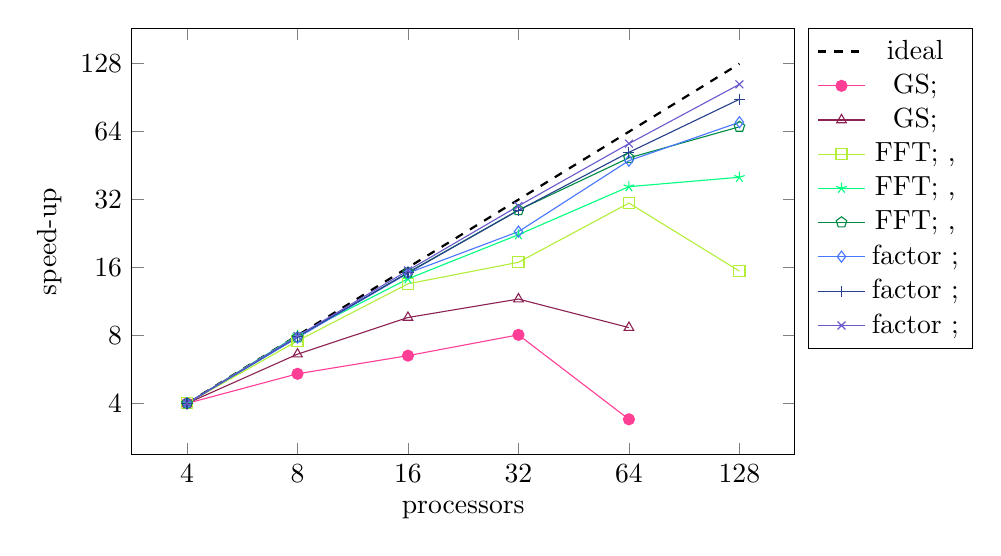
\begin{tikzpicture}
\begin{loglogaxis}[width=10cm, height=7cm, xlabel=processors, ylabel=speed-up,
xtick={4,8,16,32,64,128}, ytick={4,8,16,32,64,128}, xticklabels={4,8,16,32,64,128}, yticklabels={4,8,16,32,64,128}]
\addplot[color=black, thick, dashed] coordinates {(4,4) (128,128)};
\addlegendentry{ideal};

\addplot[color=VioletRed1, mark=*] coordinates {(4,4) (8, 5.41) (16, 6.51) (32, 8.05) (64, 3.4)};
\addlegendentry{GS; };

\addplot[color=VioletRed4, mark=triangle] coordinates {(4,4) (8, 6.61) (16, 9.61) (32, 11.6) (64, 8.67)};
\addlegendentry{GS; };

\addplot[color=OliveDrab2, mark=square] coordinates {(4,4) (8, 7.57) (16, 13.55) (32, 16.88) (64, 30.89) (128, 15.43)};
\addlegendentry{FFT; , };

\addplot[color=SpringGreen1, mark=star] coordinates {(4,4) (8, 8.01) (16, 14.26) (32, 22.37) (64, 36.53) (128, 40.2)};
\addlegendentry{FFT; , };

\addplot[color=SpringGreen4, mark=pentagon] coordinates {(4,4) (8, 7.84) (16, 15.21) (32, 28.76) (64, 48.99) (128, 67.28)};
\addlegendentry{FFT; , };

\addplot[color=RoyalBlue1, mark=diamond] coordinates {(4,4) (8, 7.83) (16,15.12) (32, 23.08) (64, 47.63) (128, 70.49)};
\addlegendentry{factor ; };

\addplot[color=RoyalBlue4, mark=+] coordinates {(4, 4) (8, 7.91) (16, 15.15) (32, 28.69) (64, 51.84) (128, 89.11)};
\addlegendentry{factor ; };

\addplot[color=SlateBlue3, mark=x] coordinates {(4,4) (8, 7.96) (16, 15.53) (32, 30) (64, 56.66) (128, 103.8)};
\addlegendentry{factor ; };
\end{loglogaxis}
\end{tikzpicture}
\caption{Parallel speed-up of various processes on the XMT.  For all runs, take .}
\label{factorr}
\end{figure}

The overall speed-up of the algorithm is shown in Figure \ref{ovef}.   We saw excellent scaling by the time we reached , except for on 128 processors where the FFT began performing much worse.  This did not happen for   and thus we expect that a more optimized FFT implementation would avoid this issue entirely.  Table 1 shows the overall runtime in seconds for the various processes on each of the runs shown in Figure \ref{ovef}; similarly, Table 2 gives the results for the Gram-Schmidt process, Table 3 for the FFT, and Table 4 for the factorization of .    We did not run the code on either 1 or 2 processors due to constraints on our benchmarking time, and due to the excellent scaling of nearly all of the steps of the algorithm in between 4 and 8 processors.  

\begin{figure}
\centering
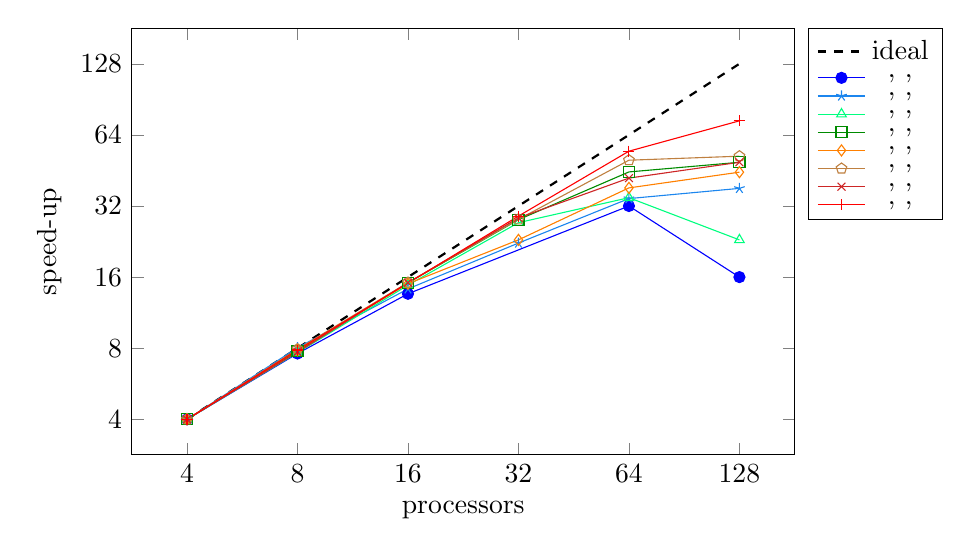
\begin{tikzpicture}
\begin{loglogaxis}[width=10cm, height=7cm, xlabel=processors, ylabel=speed-up,
xtick={4,8,16,32,64,128}, ytick={4,8,16,32,64,128}, xticklabels={4,8,16,32,64,128}, yticklabels={4,8,16,32,64,128}]
\addplot[color=black, thick, dashed] coordinates {(4,4) (128,128)};
\addlegendentry{ideal};

\addplot[color=blue, mark=*] coordinates {(4,4) (8, 7.6) (16, 13.6)  (64, 32) (128, 16)};
\addlegendentry{, , };

\addplot[color=DodgerBlue2, mark=star] coordinates {(4,4) (8, 8.04) (16, 14.26)  (32, 22.3) (64, 34.4) (128, 38)};
\addlegendentry{, , };

\addplot[color=SpringGreen1, mark=triangle] coordinates {(4,4) (8, 7.66) (16, 14.8)  (32, 27.2) (64, 34.7) (128, 23)};
\addlegendentry{, , };

\addplot[color=Green4, mark=square] coordinates {(4,4) (8, 7.78) (16, 15.14)  (32, 28) (64, 44.6) (128, 49)};
\addlegendentry{, , };

\addplot[color=orange, mark=diamond] coordinates {(4,4) (8, 7.84) (16, 15)  (32, 23) (64, 38.18) (128, 44.5)};
\addlegendentry{, , };

\addplot[color=brown, mark=pentagon] coordinates {(4,4) (8, 7.93) (16, 15.17)  (32, 28.1) (64, 50) (128, 52)};
\addlegendentry{, , };

\addplot[color=Firebrick3, mark=x] coordinates {(4,4) (8, 7.7) (16, 15.15)  (32, 28.5) (64, 42) (128, 49)};
\addlegendentry{, , };

\addplot[color=red, mark=+] coordinates {(4,4) (8, 7.86)  (32, 29) (64, 54.6) (128, 73.4)};
\addlegendentry{, , };

\end{loglogaxis}
\end{tikzpicture}
\caption{Parallel speed-up of the overall algorithm on the XMT.  For all runs, take .}
\label{ovef}
\end{figure}

\begin{table}[here]
\centering
\begin{tabular}{|c|c|c|c|c|c|c|}\hline
matrix parameters &\ 4 &\ 8 &\ 16 &\ 32 &\ 64 &\ 128  \\ \hline
, ,  &\ 56.0 &\ 29.56  &\  16.61  &\  13.37 &\  7.16  &\ 14.04  \\ 
, ,  &\  188.6 &\ 95.2  &\ 53.52  &\ 34.1  &\ 21.88   &\  20.46  \\ 
, ,  &\ 381.1   &\  194.7 &\  103.3   &\  56.43   &\  44.2  &\  68.4  \\ 
, ,  &\ 923.9  &\  476.1 &\  244.7 &\ 133.6  &\  84.12  &\  76.83 \\ 
, ,  &\  732.8 &\  375.4 &\ 196.5  &\  129.4 &\  77.16   &\ 67.87  \\ 
, ,  &\   5657 &\  2873 &\ 1492  &\  806.6 &\   455.3 &\  444.01 \\ 
, ,  &\ 3780  &\  1919 &\   1001 &\  531.4 &\  363.9   &\  310  \\ 
, ,  &\  20167 &\ 10233 &\  -- &\  2894 &\    1479 &\  1099  \\  \hline
\end{tabular}
\caption{Runtime of the total algorithm, in seconds, for the given parameters and number of processors listed in the top row.}
\label{bigt}
\end{table}

\begin{table}[here]
\centering
\begin{tabular}{|c|c|c|c|c|c|c|}\hline
matrix parameters &\ 4 &\ 8 &\ 16 &\ 32 &\ 64 &\ 128  \\ \hline
, ,  &\ 43.0 &\ 22.7 &\ 12.69  &\  10.9 &\  5.57  &\   11.15 \\ 
, ,  &\  176.0 &\ 88.4 &\  49.63 &\  31.65 &\    19.4 &\  17.61 \\ 
, ,  &\  175.4  &\  88.4 &\  46.76  &\  25.85 &\   19.6 &\  17.70 \\ 
, ,  &\  718.0  &\ 363.4  &\  188.1  &\ 99.44   &\  60.86   &\ 42.23  \\ 
, ,  &\  684.3 &\  350.5 &\  183.3 &\  122.2 &\  72.39  &\  63.7  \\ 
, ,  &\   687.8  &\  350.93 &\  183.82 &\ 114.9  &\  59.82   &\  64.71  \\ 
, ,  &\  683.6 &\ 360 &\  199.5  &\  114.3  &\  137.15  &\  148.1  \\ 
, ,  &\  691  &\  362 &\  -- &\   123.9 &\   79.91 &\ 168  \\  \hline
\end{tabular}
\caption{Runtime of the FFT, in seconds, for the given parameters and number of processors listed in the top row.  Note that this is effectively independent of .}
\label{bigt1}
\end{table}
\begin{table}[here]
\centering
\begin{tabular}{|c|c|c|c|c|c|c|}\hline
matrix parameters &\ 4 &\ 8 &\ 16 &\ 32 &\ 64 &\ 128  \\ \hline
, ,  &\ 0.23 &\ 0.36 &\  0.43 &\  0.53  &\  0.52   &\  2.11 \\ 
, ,  &\  0.23  &\  0.35 &\  0.44  &\  0.46 &\  1.41   &\  2.09  \\ 
, ,  &\  6.80 &\ 5.03 &\ 4.19  &\  3.38 &\   8.00 &\  39.3  \\ 
, ,  &\  6.86 &\  4.16 &\  4.12 &\   3.82 &\  6.66  &\ 23.2  \\ 
, ,  &\  0.22 &\ 0.24  &\ 0.39   &\  0.52 &\  1.04   &\ 2.0  \\ 
, ,  &\  83.2 &\ 50.11  &\  34.65 &\  28.7 &\ 38.4   &\  175.9 \\ 
, ,  &\  6.66 &\  4.88 &\ 3.74  &\  3.61  &\    7.19 &\  42.74  \\ 
, ,  &\ 82.02  &\  49.69 &\  --  &\  30.8 &\   29.32 &\  183.9 \\  \hline
\end{tabular}
\caption{Runtime of the Gram-Schmidt process, in seconds, for the given parameters and number of processors listed in the top row.   Note that it is effectively independent of  and .}
\label{bigt2}
\end{table}
\begin{table}[here]
\centering
\begin{tabular}{|c|c|c|c|c|c|c|}\hline
matrix parameters &\ 4 &\ 8 &\ 16 &\ 32 &\ 64 &\ 128  \\ \hline
, ,  &\ 12.5 &\ 6.50 &\  3.49  &\  1.93 &\   1.07 &\  0.78 \\ 
, ,  &\  12.4 &\ 6.47  &\  3.45  &\ 1.94   &\  1.07   &\  0.76  \\ 
, ,  &\  198.9  &\ 101.3  &\   52.3 &\  27.2 &\  16.6  &\  11.4 \\ 
, ,  &\  199.0 &\  108.5 &\  52.52   &\ 30.3  &\   16.6 &\  11.4 \\ 
, ,  &\  48.3 &\  24.65 &\  12.78  &\   6.74 &\   3.73 &\  2.17 \\ 
, ,  &\  4886 &\ 2463 &\  1274  &\  663  &\  357.1  &\  203.4 \\ 
, ,  &\ 3090  &\ 1554  &\ 797.3  &\ 413.5  &\   219.5 &\  119.2 \\ 
, ,  &\  19394  &\ 9821  &\  --  &\ 2739   &\ 1370   &\  747   \\  \hline
\end{tabular}
\caption{Runtime of the factorization of  and , in seconds, for the given parameters and number of processors listed in the top row.  Note that this is effectively independent of .}
\label{bigt3}
\end{table}


As a final note, it is worthwhile to emphasize that as our benchmarking spanned an order of magnitude in matrix size, the increase in error on average was similarly an magnitude: from about  to .  Thus, we have found that the numerically determined low bounds on the error in this algorithm continue to hold on much larger matrices (recall that the proof of the error bound relied on a slightly different randomization scheme).  Table \ref{ertab} shows the errors bounds for some sample runs.  We found, as in \cite{rokpnas}, that the numerical error bound is satisfied, although reasonably tightly.  
\begin{table}[here]
\centering
\begin{tabular}{|c|c|}\hline
matrix parameters &\  \\ \hline
, ,  &\  \\
, ,  &\  \\
, ,  &\  \\
, ,  &\  \\
, ,  &\  \\
, ,  &\  \\
, ,  &\  \\
, ,  &\  \\ \hline
\end{tabular}
\caption{The error, , for a variety of runs on the XMT.  Note that we would expect  to be of the order , and thus  if our bound was tight.  For the larger matrices these spectral norm bound increases by a  factor of 8.}
\label{ertab}
\end{table}

As mentioned in the introduction, we are not aware that randomized algorithms have been tested on such large matrices using highly parallel implementations to date.   \cite{konda} presents an algorithm for a fast parallel SVD on bidiagonal matrices which obtains similar speed-ups to ours, although our algorithm works on any low rank matrix.

\section{Conclusion}
This letter demonstrates that the parallel implementations of randomized algorithms are efficient and scale well for very large matrices.  These algorithms do tend to become less ideal on 128 processors because the FFT is starved, but we emphasize that as our results can be obtained for \emph{arbitrary} matrices with low rank, even the scaling we found is very impressive.  

Furthermore, concerns about the breakdown of the randomized algorithm on large matrices approaching are unfounded -- we have demonstrated that the error in the algorithms slowly enough with matrix size that they should be adequate for many applications.  Finally, we stress that our benchmarking was done on dense random matrices -- it is quite likely that the scaling would be far better were the low rank matrices in question of a more specialized form where certain steps in the algorithm could be optimized further.

Optimizing the Gram-Schmidt and FFT algorithms on highly parallel architectures is an active area of research and it is almost assured that specialized code would be  faster than ours on these components.  However we did not feel it appropriate to emphasize the optimization of these algorithms in the preparation of this letter, as our focus was instead on the parallelization of randomized algorithms.  Work on improving these components of the algorithm, as well as finding specialized random algorithms for certain classes of large (low-rank) matrices is a worthwhile direction for future research.

\section*{Acknowledgements}
\addcontentsline{toc}{section}{Acknowledgements}
The authors would like to thank the staff at CACR for help with initial benchmarking of the algorithm and for advice on optimization, as well as the staff at PNNL for assistance and usage of the Cray XMT.   We would also like to thank V. Rokhlin for helpful comments.

\bibliographystyle{unsrt}
\addcontentsline{toc}{section}{References}
\bibliography{xmtmatrixbib}

\end{document}
